% !TeX root = tcolorbox.tex
% include file of tcolorbox.tex (manual of the LaTeX package tcolorbox)
% \clearpage

% Initialization Option Keys
\section{初始化选项}\label{sec:initkeys}%
\tcbset{external/prefix=external/initoptions_}%
\begin{stripedbox}
The \emph{initialization} options are only applicable for the generation
of new environments and commands based on |tcolorbox| and friends.
Particularly, they can be used for
\tcblower
\emph{initialization}选项只适用于生成的新环境和基于|tcolorbox|之类的命令。%
特别是,它们可以用于
\end{stripedbox}

\begin{itemize}
\item\refComLe{newtcolorbox},
\item\refComLe{newtcbox},
\item\refComLe{newtcblisting},
\item\refComLe{newtcbinputlisting},
\item\refComLe{newtcbtheorem}, and
\item\refComLe{newtcboxfit}.
\end{itemize}

\bigskip
\begin{marker}
\begin{stripedbox}[blank]
Typically, these options may generate counters and alike.
It is \textbf{strongly} recommended that you use initialization options inside the preamble only. 
Otherwise, you may get trouble when using \LaTeX's |\include| features.
Also, it is recommended to generate new environments and commands with these
options \emph{after} |hyperref| is loaded to avoid warnings about \emph{duplicate identifiers}.
\tcblower
通常,这些选项可能用于生成计数器等。%
\textbf{强烈}建议只在序言中使用初始化选项。%
否则,在使用\LaTeX 的|\include|特性时可能会遇到麻烦。
此外,建议在 |hyperref| 加载\emph{之后}才使用这些选项来生成新的环境和命令,以避免关于\emph{duplicate identifiers}的警告。
\end{stripedbox}
\end{marker}


% Numbered Boxes
\subsection{为盒子编号}\label{sec:numberedboxes}
\begin{stripedbox}
Counters assigned using the initialization options are administrated automatically.
Especially, they are increased for each new box.
Independent from the real counter name, 
the counter value can be referenced by \docAuxCommand{thetcbcounter}, e.\,g.\ 
inside the title of the box. 
The real counter name is stored inside \docAuxCommand{tcbcounter}.
\tcblower
使用初始化选项分配的计数器将被自动管理。%
特别是,每增加一个新盒子,计数器的值就会增加。%
不依赖于具体的真实的计数器名,盒子的计数器值可以由\docAuxCommand{thetcbcounter}取得, e.\,g.\ %
在盒子的标题里面。%
真正的计数器名称存储在\docAuxCommand{tcbcounter}中。
\end{stripedbox}


\begin{newTcbKey}{auto counter}{}{no value, initially unset}
\begin{stripedbox}
Creates a new counter automatically.%
With \refKeyLe{/tcb/new/number format} and \refKeyLe{/tcb/new/number within}, 
the appearance and behavior of the counter can be changed. 
The counter value is referenced by \docAuxCommand{thetcbcounter}.
\tcblower
自动创建一个新的计数器。%
使用 \refKeyLe{/tcb/new/number format} 和 \refKeyLe{/tcb/new/number within}, %
可以更改计数器的外观和行为。%
计数器值可以由\docAuxCommand{thetcbcounter}取得。
\end{stripedbox}


\inputpreamblelisting{A}

% This box is automatically numbered with \ref{myautocounter} on page \pageref{myautocounter}. 
% Inside the box, the \thetcbcounter\ can also be referenced by |\thetcbcounter|.
% The real counter name is \texttt{\tcbcounter}.
\begin{dispExample}
\begin{pabox}[label={myautocounter}]{带编号的标题}
这个盒子是自动编号的,来自第 \pageref{myautocounter} 页的 \ref{myautocounter}。%
在盒子内部,引用 \thetcbcounter\ 可以使用 |\thetcbcounter| 生成。
真正的计数器名称是\texttt{\tcbcounter}。
\end{pabox}
\end{dispExample}
\end{newTcbKey}


% \clearpage
\begin{newTcbKey}{use counter from}{=\meta{tcolorbox}}{no default, initially unset}
\begin{stripedbox}
Here, a counter from another \meta{tcolorbox} is reused.
Note that the settings for 
\refKeyLe{/tcb/new/number format} and \refKeyLe{/tcb/new/number within} 
are inherited and cannot be changed.
The counter value is referenced by \docAuxCommand{thetcbcounter}.
\tcblower
这里,来自另一个\meta{tcolorbox}的计数器被重用。%
注意,\refKeyLe{/tcb/new/number format} 和 \refKeyLe{/tcb/new/number within} 的设置是继承的,不能更改。%
计数器值可以从 \docAuxCommand{thetcbcounter} 取得。
\end{stripedbox}

\begin{dispExample}
\newtcolorbox[use counter from=pabox]{mybox}[2][]{%
colback=blue!5!white,colframe=blue!75!black,fonttitle=\bfseries,
title=Some Box \thetcbcounter: #2,#1}
% 第一个默认参数为空,用于指定额外的选项
% 第二个参数用于指定标题内容
\begin{mybox}[label={myusecounterfrom}]{Title with continued number}
这个盒子是自动编号的,来自第 \pageref{myusecounterfrom} 页的 \ref{myusecounterfrom} 小节。
在盒子内部,引用 \thetcbcounter\ 可以使用 |\thetcbcounter| 生成。%
真正的计数器名称是 \texttt{\tcbcounter}.
\end{mybox}
\end{dispExample}
\end{newTcbKey}

\begin{newTcbKey}{use counter}{=\meta{counter}}{no default, initially unset}
\begin{stripedbox}
Here, an ordinary existing \LaTeX\ \meta{counter} is used for numbering.
With \refKeyLe{/tcb/new/number format} and \refKeyLe{/tcb/new/number within}, 
the appearance and behavior of the counter can be changed. 
The counter value is referenced by \docAuxCommand{thetcbcounter}.
\tcblower
%这里,
使用已经存在的 \LaTeX\ 计数器 \meta{counter} 来编号。%
使用 \refKeyLe{/tcb/new/number format} 和 \refKeyLe{/tcb/new/number within}, %
可以更改计数器的外观和行为。%
计数器值可以由\docAuxCommand{thetcbcounter}取得。
\end{stripedbox}    


\begin{dispExample}
% \newcounter{myexample}%  preamble
\newtcolorbox[use counter=myexample,number format=\Alph]{mybox}[2][]{%
colback=green!5!white,colframe=green!55!black,fonttitle=\bfseries,
title=Some Box \thetcbcounter: #2,#1}

\begin{mybox}[label={myusecounter}]{Title with \LaTeX\ number}
这个盒子自动编号,位于 \pageref{myusecounter} 页第 \ref{myusecounter} 小节。%
在盒子内部,引用 \thetcbcounter\ 可以使用 |\thetcbcounter| 生成。%
真正的计数器名称是\texttt{\tcbcounter}。
\end{mybox}
\end{dispExample}
\end{newTcbKey}


\begin{newTcbKey}[][doc new=2014-09-19]{use counter*}{=\meta{counter}}{no default, initially unset}
\begin{stripedbox}
An existing \LaTeX\ \meta{counter} is used for numbering. 
In contrast to \refKeyLe{/tcb/new/use counter}, the options \refKeyLe{/tcb/new/number format} and
\refKeyLe{/tcb/new/number within} are ignored. 
Use this for counters which are already configured outside the |tcolorbox| package, e.\,g.\ the standard |figure| counter.
\tcblower
使用已经存在的 \LaTeX\ 计数器 \meta{counter} 来编号。%
同 \refKeyLe{/tcb/new/use counter} 相反, 选项 \refKeyLe{/tcb/new/number format} 和 \refKeyLe{/tcb/new/number within} 被忽略。%
这用于使用在 |tcolorbox| 包外定义的计数器, e.\,g.\ 标准的 |figure| 计数器。
\end{stripedbox}
\end{newTcbKey}

\begin{newTcbKey}{no counter}{}{no value, initially set}
\begin{stripedbox}
The created boxes are not numbered. This is the default. 
The option may be used to overrule a previous option.
\tcblower
创建的盒子没有编号。这是默认值。%
该选项可用于否决先前的选项。
\end{stripedbox}
\end{newTcbKey}

% \enlargethispage*{1cm}

\begin{newTcbKey}[][doc new=2019-10-18]{reset counter on overlays}{\colOpt{=true\textbar false}}{default |true|, initially |false|}
\begin{stripedbox}
For |beamer| slides, this invokes the |\resetcounteronoverlays| command for the box counter. 
The counter is automatically reset on subsequent overlay slides of a frame.
Thereby, the counter will be the same on all slides of every frame.
\tcblower
%to 再翻译
对于|beamer|幻灯片,这为盒子计数器调用|\ resetcounteronoverlay|命令。
计数器在帧的后续覆盖幻灯片上自动重置。
因此,计数器在每一帧的所有幻灯片上都是相同的。
\end{stripedbox}
\end{newTcbKey}

% \clearpage
\begin{newTcbKey}{number within}{=\meta{counter}}{no default, initially unset}
\begin{stripedbox}
The automatic counter is set to zero, if \meta{counter} is increased.
Additionally, during output, 
the value of \meta{counter} is prepended to the value of the automatic counter.\par
To prepend the automatic counter with the chapter number and to reset it with every new chapter, use:
\tcblower
如果\meta{counter}增加,则自动计数器被设置为零\footnote{译注,类似于section计数器在chapter计数器增加时会重置的效果一样。}。
\meta{counter}的值被加在盒子自动计数器的值之前。\par
要在自动计数器前加上章节号,并在每一个新的章节中重置它,请使用:
\end{stripedbox}

\begin{dispListing}
number within=chapter
\end{dispListing}
\begin{stripedbox}
See \refKeyLe{/tcb/new/use counter} for a complete example.
\tcblower
完整的示例请参见\refKeyLe{/tcb/new/use counter}。
\end{stripedbox}
\end{newTcbKey}


\begin{newTcbKey}{number format}{=\meta{format macro}}{no default, initially \texttt{\textbackslash arabic}}
\begin{stripedbox}
Declares the format of the automatic counter. 
The \meta{format macro} can be any valid \LaTeX\ number formatting macro like |\arabic|, |\roman|, etc.\par
To display the counter value in large roman numbers, use:
\tcblower
声明自动计数器的格式。%
\meta{format macro}可惜是任何合法的 \LaTeX\ 数字格式化宏命令,比如像 |\arabic|, |\roman|, 等等。\par
要以大罗马数字显示计数器值,请使用:
\end{stripedbox}

\begin{dispListing}
number format=\Roman
\end{dispListing}
\begin{stripedbox}
See \refKeyLe{/tcb/new/auto counter} for a complete example.
\tcblower
完整的示例请参见\refKeyLe{/tcb/new/auto counter}。
\end{stripedbox}
\end{newTcbKey}

\begin{newTcbKey}{number freestyle}{=\meta{code}}{no default, initially unset}
\begin{stripedbox}
Allows advanced control over the complete number format.%
This option overrules the format given by \refKeyLe{/tcb/new/number within} and \refKeyLe{/tcb/new/number format}.
Nevertheless, you can combine it with \refKeyLe{/tcb/new/number within} to get the desired reset property.\par
The \meta{code} is some formatting code which should contain |\tcbcounter| to reference the automated counter.
Since this \meta{code} is expanded, you have to secure each macro with |\noexpand| with \emph{exception} of |\tcbcounter|.
\tcblower
允许对完整的数字格式进行高级控制。%
该选项会推翻\refKeyLe{/tcb/new/number within}和\refKeyLe{/tcb/new/number format}给出的格式。
不过,你可以将它与\refKeyLe{/tcb/new/number within}结合起来,以获得所需的重置属性。\par
\meta{code}是一些格式化代码,可以包含|\tcbcounter|来引用自动计数器。
由于这个\meta{code}是展开的,\emph{除了} |\tcbcounter| 外,你必须用 |\noexpand| 来保护每个命令。
\end{stripedbox}

\inputpreamblelisting{H}

\begin{dispExample}
\begin{phbox}[label={myfreestyle}]{编号是myfreestyle的标题}
这个盒子自动编号,位于 \pageref{myfreestyle} 页 \ref{myfreestyle}。%
在盒子内部,引用 \thetcbcounter\ 可以使用 |\thetcbcounter| 生成。%
真正的计数器名称是\texttt{\tcbcounter}。
\end{phbox}
\end{dispExample}
\end{newTcbKey}

% \clearpage
\begin{marker}
\begin{stripedbox}[blank]
The following options \refKeyLe{/tcb/new/crefname} and \refKeyLe{/tcb/new/Crefname}
need to be set inside the preamble.
\tcblower
以下选项\refKeyLe{/tcb/new/crefname}和\refKeyLe{/tcb/new/crefname}需要设置在导言区内。
\end{stripedbox}
\end{marker}

\begin{newTcbKey}[][doc updated=2014-12-01]{crefname}{=\marg{singular}\marg{plural}}{no default, initially unset}
\begin{stripedbox}
This option key can be used only in conjunction with the |cleveref| package
%\cite{cubitt:2018a} 
which has to be loaded separately.
It creates a cross-reference type for the new |tcolorbox|'es, where the
lowercase \meta{singular} and \meta{plural} forms of the cross-reference are given.
This type is the environment or macro name and \refKeyLe{/tcb/label type} is set automatically.
See \refKeyLe{/tcb/label type} and \cite{cubitt:2018a} 
for more information.
\tcblower
此选项只能与~|cleveref|~包结合使用。%,必须分开装载。
%\cite{cubitt:2018a} 
它为新的 |tcolorbox|'es 创建了一个交叉引用类型, %
其中给出了交叉引用的小写的 \meta{singular}(单数) 和 \meta{plural}(复数)形式。%
该类型是环境或宏名称,会自动设置\refKeyLe{/tcb/label type}。%
更多信息请参见 \refKeyLe{/tcb/label type} 和 \cite{cubitt:2018a}。
\end{stripedbox}
\end{newTcbKey}

\begin{newTcbKey}[][doc updated=2014-12-01]{Crefname}{=\marg{singular}\marg{plural}}{no default, initially unset}
\begin{stripedbox}
This option key can be used only in conjunction with the |cleveref| package
\cite{cubitt:2018a} which has to be loaded separately.
It creates a cross-reference type for the new |tcolorbox|'es, where the
uppercase \meta{singular} and \meta{plural} forms of the cross-reference are given.
This type is the environment or macro name and \refKeyLe{/tcb/label type} is set automatically.
See \refKeyLe{/tcb/label type} and \cite{cubitt:2018a} for more information.
\tcblower
此选项只能与~|cleveref|~包结合使用。%,必须分开装载。
它为新的 |tcolorbox|'es 创建了一个交叉引用类型, %, where the
其中给出了交叉引用的大写的 \meta{singular}(单数) 和 \meta{plural}(复数)形式。%
该类型是环境或宏名称,会自动设置\refKeyLe{/tcb/label type}。%
更多信息请参见 \refKeyLe{/tcb/label type} 和 \cite{cubitt:2018a}。
\end{stripedbox}
\end{newTcbKey}

\inputpreamblelisting{I}
\begin{dispExample}
% \usepackage{varioref}
% \usepackage{cleveref}
\begin{mybluebox}[label={myreference}]{我的标题}
This is an example.
\end{mybluebox}

大写的引用类型名加计数引用,|\Cref{myreference}|:\Cref{myreference},\\ 
小写的引用类型名加计数引用,|\cref{myreference}|:\cref{myreference}.\\

大写的前缀加页数计数器值,|\Cpageref{myreference}|:\Cpageref{myreference}\\
小写的前缀加页数计数器值,|\cpageref{myreference}|:\cpageref{myreference} .\\

大写的引用类型,|\nameCref{myreference}|:\nameCref{myreference}\\
小写的引用类型,|\namecref{myreference}|:\namecref{myreference}\\

计数引用,|\labelcref{myreference}|:\labelcref{myreference}\\
页数,|\labelcpageref{myreference}|:\labelcpageref{myreference}\\

With \texttt{varioref}:\\
大写的引用类型名加计数引用,|\Vref{myreference}|:\Vref{myreference}\\
小写的引用类型名加计数引用,|\vref{myreference}|:\vref{myreference}\\

大写的引用类型名加计数引用,|\Vref*{myreference}|:\Vref*{myreference}\\
小写的引用类型名加计数引用,|\vref*{myreference}|:\vref*{myreference}.
\end{dispExample}

% \clearpage

\begin{newTcbKey}[][doc new=2014-09-19]{blend into}{=\meta{name}}{style, no default, initially unset}
\begin{stripedbox}
Used to comfortably blend into an existing schema of naming and numbering for
some selected cases. For example, a |tcolorbox| can be used to display
and entitle an image pretending to be a standard |figure| environment.
Here, \refKeyLe{/tcb/title} is used instead of the standard |\caption|
and \refKeyLe{/tcb/list text} can be used instead of the optional parameter
of the standard |\caption|.
\tcblower
用于对某些选定的情况, 轻松地混合到现有的命名和编号模式中。%
例如,|tcolorbox| 可用于显示并赋予图像标题,假装是标准~|figure|~环境。%
这里使用了\refKeyLe{/tcb/title}来代替标准的|\caption|,%
而\refKeyLe{/tcb/list text}可以用来代替标准 |\caption| 的可选参数。%
\end{stripedbox}

\begin{stripedbox}
Feasible values for \meta{name} are:
\tcblower
\meta{name}的可行值是:
\end{stripedbox}
\begin{itemize}
\item\docValue{figures}: 
\begin{stripedbox}%[width=\linewidth]
blend into the standard |figure| environment.
\tcblower
融入标准 |figure| 环境。
\end{stripedbox}

\item\docValue{tables}:
\begin{stripedbox}
blend into the standard |table| environment.
\tcblower
融入标准 |table| 环境。
\end{stripedbox}
\item\docValue{listings}: 
\begin{stripedbox}
blend into the standard |lstlisting| environment
of the package |listings| %\cite{hoffmann:listings}
.
\tcblower
融入 |listings| 包的 |lstlisting| 环境。
\end{stripedbox}

\begin{marker}
\begin{stripedbox}[blank]
Note that |blend into=listings| can only be used in the document content
or, preferably, inside a |\AtBeginDocument| clause! Using it without
|\AtBeginDocument| inside the preamble does not work since the |listings|
packages initializes its counter also inside |\AtBeginDocument|.
\tcblower
注意,|blend into=listings| 只能在文档内容中使用,%
或者,最好是在 |\AtBeginDocument| 中!%
在导言区中而不是在 |\AtBeginDocument| 中的话,是不工作的,%
因为 |listings| 包初始化它的计数器也在 |\AtBeginDocument| 里。
\end{stripedbox}
\end{marker}
\end{itemize}
\end{newTcbKey}

% \enlargethispage*{5cm}
\begin{dispListing}
\begin{figure}[htb]
  \centering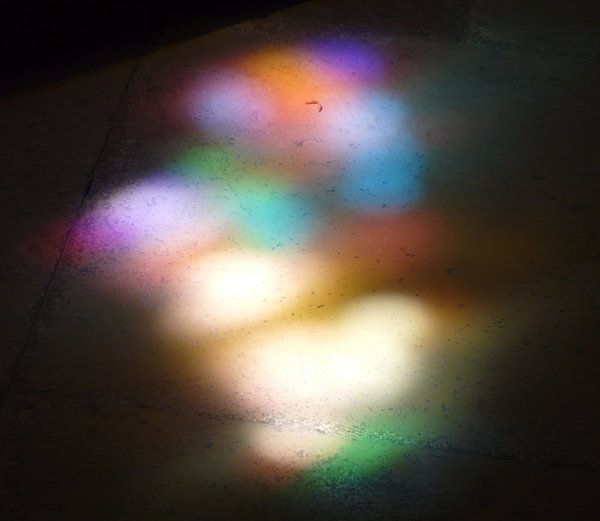
\includegraphics[height=4cm]{lichtspiel.jpg}
  \caption{标准的figure}
\end{figure}

\newtcolorbox[blend into=figures]{myfigure}[2][]{float=htb,capture=hbox,
  title={#2},every float=\centering,#1}

\begin{myfigure}{tcolorbox的figure}
  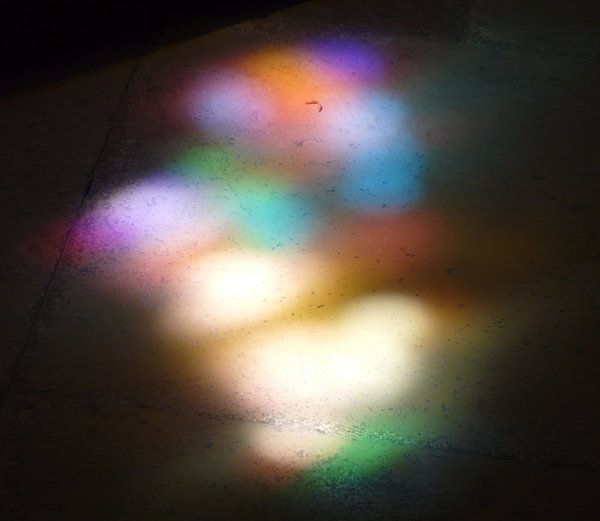
\includegraphics[height=4cm]{lichtspiel.jpg}
\end{myfigure}
\end{dispListing}
{\tcbusetemp}

% \clearpage
\begin{docTcbKey}[][doc new=2015-03-13]{blend before title}{=\meta{value}}{no default, initially \docValue{colon}}
\begin{stripedbox}
This option formats the title output of \refKeyLe{/tcb/new/blend into}.
Note that this is a common |tcolorbox| option which should be set
globally or in the normal option part of \refComLe{newtcolorbox}.
\tcblower
该选项用于格式化\refKeyLe{/tcb/new/blend into}的标题输出。%
注意,这是一个常见的 |tcolorbox| 选项,应该全局设置, 或在 \refComLe{newtcolorbox} 的普通选项部分。\end{stripedbox}

\begin{stripedbox}
Feasible values for \meta{value} are:
\tcblower
\meta{value}的可行值是:
\end{stripedbox}
\begin{itemize}
\item\docValue{colon}: 
\begin{stripedbox}
use name/number plus colon.
\tcblower
使用 |名字|/|编号| 加上 |冒号|
\end{stripedbox}

\item\docValue{dash}: 
\begin{stripedbox}
use name/number plus dash.
\tcblower
使用 |名字|/|编号| 加上 |破折号|
\end{stripedbox}

\item\docValue{colon hang}: 
\begin{stripedbox}
use name/number plus colon with hanging indent.
\tcblower
使用 |名字|/|编号| 加上 |冒号|,并悬挂式缩进。
\end{stripedbox}

\item\docValue{dash hang}: 
\begin{stripedbox}
use name/number plus dash with hanging indent.
\tcblower
使用 |名字|/|编号| 加上 |破折号|,并悬挂式缩进。
\end{stripedbox}
\end{itemize}

\begin{dispListing}
\newtcolorbox[blend into=figures]{myfigure}[2][]{float=htb,capture=hbox,
  blend before title=dash hang,title={#2},every float=\centering,#1}

\begin{myfigure}{一个标题相当长的tcolorbox图}
  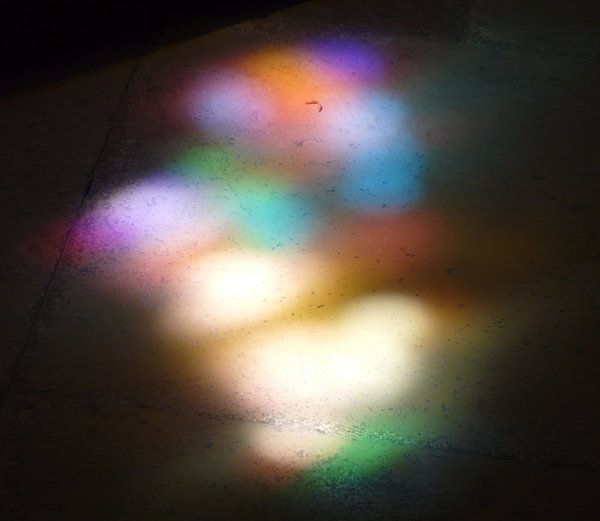
\includegraphics[height=5cm]{lichtspiel.jpg}
\end{myfigure}
\end{dispListing}
{\tcbusetemp}
\end{docTcbKey}

% \clearpage
\begin{docTcbKey}[][doc new=2015-03-13]{blend before title code}{=\meta{code}}{no default}
\begin{stripedbox}
This option formats the title output of \refKeyLe{/tcb/new/blend into}.
The \meta{code} takes one parameter, the name/number.
Use this, if \refKeyLe{/tcb/blend before title} is not flexible enough.
\tcblower
该选项格式化\refKeyLe{/tcb/new/blend into}的标题输出。%
\meta{code}接受一个参数,即 name/number。%
如果\refKeyLe{/tcb/blend before title}不够灵活,可以使用这个。
\end{stripedbox}

\begin{dispListing}
\newtcolorbox[blend into=figures]{myfigure}[2][]{float=htb,capture=hbox,
  blend before title code={\fbox{##1}\ },title={#2},every float=\centering,#1}

\begin{myfigure}{A tcolorbox figure}
  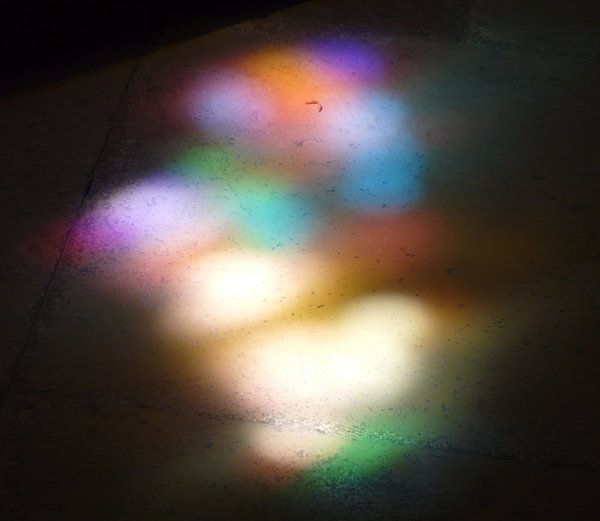
\includegraphics[height=6cm]{lichtspiel.jpg}
\end{myfigure}
\end{dispListing}
{\tcbusetemp}
\end{docTcbKey}

% \clearpage
% Lists of \texttt{tcolorbox}es
\subsection{\texttt{tcolorbox}盒子目录}\label{sec:listsof}
\begin{stripedbox}
For figures and tables, \LaTeX\ provides the |\listoffigures| and
|\listoftables| commands to create lists of these numbered entities.
Also, a |tcolorbox| can be part of such a kind of list.
\tcblower
对于图形和表格,\LaTeX\ 提供了 |\listfigures| 和 |\listoftables| 命令创建这些编号实体的列表。%
同样,|tcolorbox|可以是这种列表的一部分。
\end{stripedbox}

\begin{enumerate}
\item 
\begin{stripedbox}
Assign a list \meta{name} by the \emph{initialization} option
\refKeyLe{/tcb/new/list inside}.
\tcblower
通过\emph{初始化}选项\refKeyLe{/tcb/new/list inside}分配一个列表\meta{name}。
\end{stripedbox}

\item 
\begin{stripedbox}
Optionally, a new \meta{type} for list entries may be assigned
by the \emph{initialization} option \refKeyLe{/tcb/new/list type}.
\tcblower
可选地,通过\emph{初始化}选项\refKeyLe{/tcb/new/list type},%
可以为列表条目分配一个新的\meta{type}。
\end{stripedbox}

\item 
\begin{stripedbox}
List entries a generated automatically within each new |tcolorbox|
using the above initialization.
\tcblower
列出使用上述初始化在每个新|tcolorbox|中自动生成的条目。
\end{stripedbox}
    \begin{itemize}
    \item 
\begin{stripedbox}
If \refKeyLe{/tcb/list entry} is set, the entry is generated with it.
\tcblower
如果设置了\refKeyLe{/tcb/list entry},则生成该条目。
\end{stripedbox}
    
    \item 
\begin{stripedbox}
Otherwise, if \refKeyLe{/tcb/title} is set, the entry is generated with it.
\tcblower
否则,如果设置了\refKeyLe{/tcb/title},则生成该条目。
\end{stripedbox}
    
    \item 
\begin{stripedbox}
Otherwise, the entry is generated with the current number and the environment name.
\tcblower
否则,将使用当前编号和环境名称生成条目。
\end{stripedbox}
    
    \end{itemize}
\item 
\begin{stripedbox}
The generated list is displayed by \refComLe{tcblistof}.
\tcblower
生成的列表由\refComLe{tcblistof}显示。
\end{stripedbox}
\end{enumerate}

\begin{newTcbKey}{list inside}{=\meta{name}}{no default, initially unset}
\begin{stripedbox}
Assigns a list or contents file to the generated |tcolorbox|es.
Entries to this list are saved to a file which gets the \meta{name} as
file name extension. The list is referenced by this name in
\refComLe{tcblistof}.
For example:
\tcblower
为生成的 |tcolorbox| 盒子们分配一个列表或内容文件。%
此列表中的条目保存到一个文件中,该文件以\meta{name}作为文件扩展名。%
该列表由\refComLe{tcblistof}引用。%
例如:
\end{stripedbox}

\begin{dispListing}
list inside=exam
\end{dispListing}
\begin{stripedbox}
See Section \ref{listing:exercises} from page \pageref{listing:exercises}
for a complete example.
\tcblower
一个完整的例子参见 \pageref{listing:exercises} 页的 \ref{listing:exercises} 小节。
\end{stripedbox}
\end{newTcbKey}

\begin{newTcbKey}{list type}{=\meta{type}}{no default, initially |tcolorbox|}
\begin{stripedbox}
Optionally, some \meta{type} can be assigned to the list entries.
For a new \meta{type}, a macro |\l@|\meta{type} has to exist which controls
the format of the list entry. The default type is defined by
\tcblower
可选地,可以将列表条目设置为一些\meta{type}。%
对于一个新的\meta{type}, 存在宏命令 |\l@|\meta{type} 用于控制列表条目的格式。%
默认类型定义为:
\end{stripedbox}

\begin{dispListing}
\newcommand*\l@tcolorbox{\@dottedtocline{1}{1.5em}{2.3em}}
\end{dispListing}
\begin{stripedbox}
This is identical to the |\l@section| setting of \LaTeX. |\l@tcolorbox| can
be redefined or a new \meta{type} can be assigned.
\tcblower
这同 \LaTeX 的 |\l@section| 的定义是相同的。
|\l@tcolorbox| 可以重新定义或分配一个新的\meta{type}。
\end{stripedbox}
\end{newTcbKey}


% \clearpage
\begin{docCommand}[doc updated=2021-05-20]{tcblistof}{\oarg{macro}\marg{name}\oarg{short}\marg{title text}}
\begin{stripedbox}
Displays the generated list of |tcolorbox|es with the given \meta{name}.
The heading is generated by \meta{macro}\oarg{short}\marg{title text} where \texttt{\textbackslash section}
is the default setting for \meta{macro}.
Here, as usual, \meta{title text} is the title of the section or chapter
while \meta{short} is a shorter title for headings and table of contents.
\tcblower
用给定的\meta{name}显示生成的|tcolorbox|es列表。%
标题由\meta{macro}\oarg{short}\marg{title text}生成,其中\texttt{\textbackslash section} 是\meta{macro}的默认设置。%
这里,像往常一样,\meta{title text}是章或节的标题, \meta{short}是章或节的短标题.
\end{stripedbox}

\begin{itemize}
\item 
\begin{stripedbox}
If \meta{macro} ends with a |*|, \refComLe{tcblistof} mimics the behavior of
|\listoffigures| from the standard \LaTeX\ classes and adds the title
to the left and right mark for headings.
\tcblower
如果\meta{macro}以|*|结尾, \refComLe{tcblistof} 模拟标准 \LaTeX\ 的 |\listoffigures| 的行为,%
并将标题添加到页眉的左右标记。
\end{stripedbox}

\item 
\begin{stripedbox}
If \meta{macro} starts with |\chapter|, a possible two column document setting
is restored to one column (as standard \LaTeX\ classes do for |\listoffigures|).
\tcblower
如果\meta{macro}以|\chapter|开始, %
有一些的两列文档设置将恢复为一列 (像标准 \LaTeX\ 的 |\listoffigures| 做的那样).
\end{stripedbox}
\end{itemize}

\medskip
\begin{stripedbox}
To display the list inside a subsection, use for example:
\tcblower
要在subsection中显示列表,例如:
\end{stripedbox}
\begin{dispListing}
\tcblistof[\subsection]{exam}{List of Exercises}
\end{dispListing}
\begin{stripedbox}
The result of the example is found as Subsection \ref{listofexercises} on
page \pageref{listofexercises}.
\tcblower
示例结果可以参见在 \pageref{listofexercises} 页的 \ref{listofexercises} 小节。
\end{stripedbox}


\medskip
\begin{stripedbox}
To apply the list similar to |\listoffigures| for a report or book, use for example:
\tcblower
要将类似 |\listoffigures| 的列表应用于报告或书籍,请使用例如:
\end{stripedbox}
\begin{dispListing}
\tcblistof[\chapter*]{exam}{List of Exercises}
\end{dispListing}

\medskip
\begin{stripedbox}
To set a short title for headings with the default |\section| setting, use for example:
\tcblower
%todo 是页眉么?
使用默认|\section|设置,为页眉设置一个短标题,例如:
\end{stripedbox}
\begin{dispListing}
\tcblistof{exam}[List of Exercises]{Elaborate List of Fine Exercises
                                    for all Students of my Course}
\end{dispListing}

\medskip
\begin{marker}
\begin{stripedbox}
The core of the list is generated by |\@starttoc|\marg{name} which
can be wrapped into an own macro.
\tcblower
列表的核心是由|\@starttoc|\marg{name}生成的,%
可以包装到已有的宏。
\end{stripedbox}
\end{marker}
\end{docCommand}
